\chapter{Il livello \textit{Data-Link}}
\label{ch:livelloDataLink}

    \subsection{Introduzione}
        \paragraph{Terminologia} Definiamo gli \textit{host} e i \textit{router} come \textbf{nodi} di rete, inoltre il canale di comunicazione tra due nodi adiacenti è detto \textbf{link}. Il pacchetto di livello 2 è detto \textbf{frame}, il quale incapsula il pacchetto di livello 3, detto \textbf{datagram}.
        \paragraph{Contesto} Un percorso può essere diviso con diversi tipi di \textit{link}, un datagramma trasferito lungo un percorso attraversa la rete con protocolli di livello 2 differenti. Ad esempio su un percorso tra due nodi possono esserci link \textit{Ethernet} per il promo link, \textit{Frame Relay} per gli intermedi ed \texttt{802.11} per l'ultimo link. Ognuno dei protocolli di livello 2 fornisce servizi diversi, alcuni possono eseguire controllo di errori, altri no.
    \subsection{Servizi del livello}
        La creazione di un frame di livello 2 per l'accesso al link include:
        \begin{itemize}
            \item L'incapsulamento del datagramma in un frame, con aggiunta di un \textit{header} e un \textit{trailer}.
            \item Fornisce un meccanismo di accesso al canale condiviso, se il link è condiviso.
            \item Utilizza indirizzi di livello 2 detti \Acrshort*{MAC} negli header dei frame per identificare il mittente e il destinatario.\footnote{Gli indirizzi \Acrshort*{MAC} sono diversi dagli indirizzi \Acrshort*{IP}, i primi sono indirizzi di livello 2 e sono assegnati dal produttore della ``scheda di rete'' e dunque non possono essere cambiati, mentre gli indirizzi \Acrshort*{IP} sono assegnati dal \textit{network administrator} e possono cambiare nel tempo.}
        \end{itemize}
        Inoltre il livello 2 può fornire un servizio di consegna affidabile ai nodi adiacenti, questo spesso non viene usato per \textit{link} con basso tasso di perdita.
        \paragraph{Controllo di flusso} Il livello 2 può fornire un controllo di flusso adattando la velocità di trasmissione del mittente alla velocità accettabile del destinatario.
        \paragraph{Rilevazione di errori} Il livello 2 può rilevare errori causati da: attenuazioni, rumore e interferenze,\dots ed il ricevente può individuarne la presenza e scegliere di avvertire il mittente e/o scartare il pacchetto
        \paragraph{Corredizione di errore} Il livello 2 può correggere piccoli errori se il canale è rumoroso, ma questo è raro.
        \paragraph{\{\textit{Half}$\mid$\textit{Full\}-Duplex}} Un link può essere \textit{half-duplex} o \textit{full-duplex}, nel primo caso i due nodi possono trasmettere e ricevere, ma non contemporaneamente, nel secondo caso possono farlo contemporaneamente. Spesso si allocano due sezioni di risorse per la trasmissione e la ricezione di fatto emulando un \textit{full-duplex}.
    \subsection{Chi implementa il livello \textit{data-link}}
        Il livello \textit{data-link} è implementato da tutti gli \textit{host}, solitamente questo avviene da parte del \textit{firmware} dell'\Acrfull*{NIC} , oppure da un \textit{chip} dedicato. In ogni caso il livello \textit{data-link} è collegato direttamente al \Acrshort*{BUS} del sistema dell'\textit{host} ed è una combinazione di \textit{hardware}, \textit{software} e \textit{firmware}.
    \subsection{Comunicazione tra adattatori di rete} 
        \paragraph{Trasmissione} Quando un \textit{host} vuole trasmettere un datagramma, il livello \textit{data-link} del mittente incapsula il datagramma in un frame, aggiungendo \textit{bit} per il controllo di errore, controllo di flusso, ecc\dots e lo trasmette al \textit{link}. Il frame viene trasmesso da un adattatore di rete al \textit{link} e viene ricevuto dall'adattatore di rete del destinatario.
        \paragraph{Ricezione} L'adattatore di rete del destinatario estrae il datagramma dal frame e lo passa al livello \textit{network}. Il livello \textit{data-link} del destinatario può rilevare errori e scartare il frame se necessario.
\section{Rilevamento di errori e correzione}
    Nel datagramma vengono inseriti dei \textit{bit} \acrfull*{EDC} per rilevare e correggere errori. Questi sono \textit{bit} ridondanti che vengono aggiunti al datagramma per rilevare e correggere errori. Questi \textit{bit} sono calcolati in base ai \textit{bit} del datagramma (\texttt{D} - sia i dati che gli \textit{header}). I \textit{bit} del \Acrshort*{EDC} vengono accodati al datagramma \texttt{D} nella sua trasmissione.

    \subsection{Vari metodi per il rilevamento di errori}
        \paragraph{Controllo di parità singola} Esiste un singolo bit di parità, che viene calcolato in modo che il numero totale di \textit{bit} a 1 sia pari o dispari. Questo metodo è molto semplice e può rilevare errori singoli, ma non può correggerli e in caso di errori multipli non è in grado di rilevarli.
        \paragraph{Controllo di parità bidimensionale} Questo metodo è una generalizzazione del controllo di parità singola in questo caso si usano più bit di parità, questo sulla base di una matrice di dati, vengono usati quindi $n+m-1$ bit di parità per una matrice $n \times m$. Questo metodo può rilevare errori singoli e multipli (se non sono sulla stessa riga o colonna), ma non può correggerli, può infatti correggere solo un errore per matrice.
        \paragraph{Correzzione di errori tramite riddondanza} Semplicemente si aggiungono \textit{bit} ridondanti al datagramma, ovvero si trasmette più volte lo stesso messaggio. Questo metodo è molto costoso in termini di banda, ma permette di rilevare e correggere errori multipli.
    
    \subsection[\textit{Cyclic Redundancy Check} (\texttt{CRC})]{\acrfull*{CRC}}
        Il \Acrshort*{CRC} è il metodo più efficiente per il rilevamento di errore, considera i bit di dati come un numero binario ($D$), ed dopo aver scelto una sequenza di $r+1$ bit detto \textit{polinomio generatore} ($G$) il quale è conosciuto sia dal mittente che al destinatario. Ora il \Acrshort*{CRC} viene composto scegliendo $r$ \textit{bit} in modo che i dati $D$ siano divisibili per $G$ modulo 2 con resto $R$ (ovvero $<D,R>$ è divisibile per $G$). Se il ricevente riceve $<D',R>$ e questi non hanno resto 0, allora c'è stato un errore. A meno che non si commettano $r$ errori, il \Acrshort*{CRC} rileva tutti gli errori di lunghezza $r-1$ o meno.
        \subsubsection{Calcolo \Acrshort*{CRC}}
            \begin{enumerate}
                \item Vogliamo che valga: $D\times 2^r \operatorname{XOR} R = nG$
                \item Aggiungiamo $R$ ($\operatorname{XOR} R$) ad entrambi i lati: $D\times 2^r = nG \operatorname{XOR} R$
                \item Dunque il resto della divisione di $D\times 2^r$ per $G$ è $R$
                \item Quindi il \Acrshort*{CRC}$\rightarrow R=\operatorname{resto}\left(\frac{D\times 2^r}G\right)$
            \end{enumerate}
\section[Protocolli Accesso Multiplo Canale]{Protocolli e tecnologie per l'accesso multiplo al canale}
    \subsubsection{Tipi di collegamento}
        \paragraph{Collegamento punto-punto} Un collegamento punto-punto è un collegamento dedicato tra due nodi, questo però non è sempre rispettato a livello fisico\dots ad esempio un collegamento \textit{Ethernet} è un collegamento punto-punto, ma in realtà può essere condiviso da più nodi.
        \paragraph{Collegamento broadcast} Un collegamento broadcast è un collegamento condiviso da più nodi, i frame trasmessi da un nodo sono ricevuti da tutti gli altri nodi. Questo tipo di collegamento è tipico delle reti \Acrshort*{WLAN}.
    \subsection{Protocolli per il controllo dell'accesso multiplo}
        Questi protocolli sono tipici dei collegamenti broadcast, dove più nodi condividono lo stesso canale di trasmissione per inviare e ricevere frame. Questi protocolli si occupano di evitare che due o più trasmissioni simultanee interferiscano tra loro.
        \paragraph{Protocolli ad accesso multiplo} L'algoritmo distribuito che determina come i nodi condividono il canale, determinando quando un nodo può trasmettere. Questi accordi possono essere eseguiti sullo stesso canale (tipicamente) o su canali separati (\textit{out-of-band}).
        \subsubsection{Un protocollo \Acrshort*{MAC} ideale}
            Un protocollo \acrfull*{MAC} ideale deve, partendo da un canale \textit{broadcast} capace di supportare $R bit/s$ deve avere le seguenti caratteristiche:
            \begin{enumerate}
                \item Quando un nodo trasmette lo può fare alla velocità massima $R$.
                \item Quando $M$ nodi vogliono trasmettere, possiamo farlo ad un tasso medio pari a $R/M$.
                \item Il sistema dovrebbe essere completamente decentralizzato (senza ``centro stella'') ed inoltre non dovrebbe richiedere sincronizzazione di ``\textit{clock}''.
                \item Il protocollo deve essere semplice.
            \end{enumerate}
        \subsubsection{Protocolli \Acrshort*{MAC} realmente}
            I protocolli \Acrshort*{MAC} reali non possono soddisfare tutte le caratteristiche di un protocollo ideale, ma possono comunque essere classificati in tre categorie:
            \begin{itemize}
                \item A ripartizione delle risorse del canale
                    \subitem Dividono il canale in "sotto-canali" più piccoli ed allocando ciascuno di essi ad un nodo.
                \item Ad accesso casuale
                    \subitem I nodi trasmettono quando vogliono, ma se due nodi trasmettono contemporaneamente si verifica una collisione e i nodi devono ritrasmettere.
                \item A ``turni'' intelligenti
                    \subitem I nodi accedono al canale a turno, ma i nodi con molti dati da trasmettere possono ottenere turni più lunghi.
            \end{itemize}
    \subsection[\texttt{TDMA}, \texttt{FDMA}, \texttt{CDMA}]{\Acrshort*{TDMA}, \Acrshort*{FDMA}, \Acrshort*{CDMA}}
        \subsubsection{Ripartizione delle risorse (\Acrshort*{TDMA})}
            Il protocollo \acrfull*{TDMA} è un protocollo di accesso al canale in ``turni'' che divide il tempo in ``slot'' e assegna un ``slot'' a ciascun nodo. I nodi trasmettono solo nei loro ``slot'' assegnati. Questo protocollo è usato in reti telefoniche cellulari e satellitari.
        \subsubsection{Ripartizione delle frequenze (\Acrshort*{FDMA})}
            Il protocollo \acrfull*{FDMA} è un protocollo di accesso che prevede la divisione della banda di frequenza in ``sotto-bande'' e assegna una ``sotto-banda'' a ciascun nodo. I nodi trasmettono solo nella loro ``sotto-banda'' assegnata in qualunque momento del tempo. Questo protocollo è anche per le comunicazioni tramite mezzo coassiale.
        \subsubsection{Ripartizione del codice (\Acrshort*{CDMA})}
            Il protocollo \Acrshort*{CDMA} è un protocollo di accesso al canale che assegna un codice univoco a ciascun nodo e permette a tutti i nodi di trasmettere contemporaneamente. I nodi trasmettono i dati codificati con il loro codice univoco e i nodi riceventi decodificano i dati con il codice del mittente. Questo protocollo è usato nelle reti \Acrshort*{WLAN} e nelle reti cellulari.
        \begin{figure}[H]
            \centering
            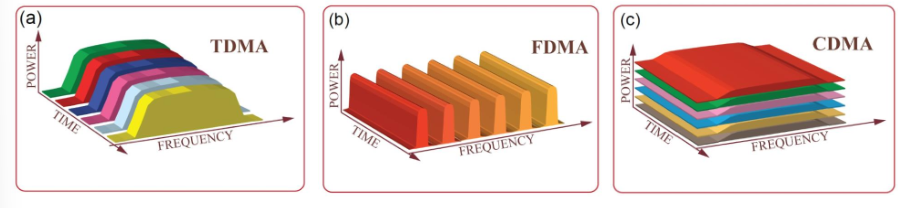
\includegraphics[width=0.8\linewidth]{05/confrontoTD-DF-CDMA.png}
            \caption{Confronto tra \Acrshort*{TDMA}, \Acrshort*{FDMA} e \Acrshort*{CDMA}}
        \end{figure}
    \subsection[\textit{Slotted ALOHA},\textit{ALOHA} Protocolli ad accesso casuale]{\Acrlong*{S-ALOHA},\Acrlong*{ALOHA} Protocolli ad accesso casuale}
            I protocolli ad accesso casuale permettono ai nodi di trasmettere quando vogliono ed alla massima velocità di trasmissione. Ma non c'è coordinamento con gli altri nodi e quindi possono verificarsi collisioni.\newline
            Un protocollo ad accesso casuale specifica: come rilevare le collisioni, come recuperare uno stato di collisione e come ritrasmettere dopo una collisione.\newline
            Alcuni esempi di accessi casuali sono: \acrfull*{S-ALOHA}, \acrfull*{ALOHA},
            \Acrshort*{CSMA}, \Acrshort*{CSMA/CD}, \Acrshort*{CSMA/CA}.
        \subsubsection{\Acrlong*{S-ALOHA}}
            Assumendo che tutti i pacchetti abbiano la stessa lunghezza e che il tempo sia diviso in "\textit{slot}" lunghi quanto un pacchetto, i nodi possono trasmettere solo all'inizio di uno slot e che i nodi siano sincronizzati. Questo protocollo allora è in collisione quando due o più nodi trasmettono nello stesso slot.
            \paragraph{Come funziona} Quando un nodo ha un pacchetto da trasmettere, lo trasmette all'inizio dello slot successivo, se non ci sono collisioni il nodo può eventualmente trasmettere un altro pacchetto. Se c'è una collisione il nodo ritrasmette il pacchetto in un altro slot con probabilità $p$ finché non riesce a trasmettere il pacchetto senza collisioni.
            \paragraph{Vantaggi} Questo protocollo molto semplice, se un solo nodo trasmette il canale è usato al 100\%, inoltre è decentralizzato e basta solo sincronizzarsi sugli slot.
            \paragraph{Svantaggi} Le collisioni sono probabili e e sprecano risorse, non sempre gli slot sono usati, potrebbero esserci collisioni senza la fine di una trasmissione, infine la sincronizzazione richiede il coordinamento.
            \paragraph{Efficienza} Assumendo che tutti i pacchetti hanno la stessa dimensione, che $G\geq 0$ sia il traffico offerto allora se $P[k]$ è la probabilità che ci siano $k$ pacchetti da trasmettete in un singolo slot, allora questa segue una \textit{distribuzione di Poisson} e la probabilità di successo è $P[k]=\frac{G^ke^{-G}}{k!}$. Dunque anche se il \textit{throughput} ideale è di $1$ il \textit{throughput} reale per un pacchetto è di $P[k=1]=Ge^{-G}$. La massima efficienza si ha per $G=1$ e dunque il massimo \textit{throughput} è di $\frac{1}{e}\stackrel{\sim}{=} 0.368$. \newline
            Supponendo di avere $N$ nodi e che ciascuno trasmette con probabilità $p$ allora la probabilità che un nodo trasmetta con successo è $p(1-p)^{N-1}$ e la probabilità che un nodo qualunque abbia successo è $\binom{N}{1}p(1-p)^{N-1} = Np(1-p)^{N-1}$. Il valore di $p$ che massimizza la probabilità di successo è $p=\frac{1}{N}$, ed il limite per $N\to\infty$ è di $\lim\limits_{N\to\infty}Np(1-p)^{N-1}=\frac{1}{e}\stackrel{\sim}{=}0.368$.
        \subsubsection{\Acrlong*{ALOHA}}
            Questo protocollo è simile al \Acrlong*{S-ALOHA}, ma è ancora più semplice in quanto non richiede la sincronizzazione sugli slot. I nodi trasmettono il prima possibile e se c'è una collisione aspettano un tempo casuale e con probabilità $p$ ritrasmettono.
            \paragraph{Efficenza} Anche in questo caso assumiamo che tutti i pacchetti abbiano la stessa dimensione e che abbiamo \textit{host} infiniti. Chiamiamo dunque $G\geq 0$ il traffico offerto la probabilità che ci siano $k$ pacchetti da trasmettere in un singolo slot è $P[k]=\frac{G^ke^{-G}}{k!}$ e il \textit{throughput} dato dalla probabilità che solo un \textit{frame} sia trasmesso nella finestra di vulnerabilità $[t_0-1,t_1+1]$ è $P[1]=Ge^{-G}$. La probabilità che non ci siano \textit{frame} trasmessi nel momento nel quale si vuole iniziare la trasmissione, ovvero nella finestra $[t_0-1,t_0]$ è $P[0]=e^{-G}$. Quindi la probabilità che un nodo trasmetta con successo è $P[k=1]\times P[k=0]=Ge^{-2G}$ il che ci porta ad un \textit{throughput} di $\frac{1}{2e}\stackrel{\sim}{=}0.184$.
    \subsection[\texttt{CSMA}, \texttt{CSMA/CD}, \texttt{CSMA/CA}]{\Acrshort*{CSMA}, \Acrshort*{CSMA/CD}, \Acrshort*{CSMA/CA}}
        \subsubsection{\acrfull*{CSMA}}
            Il protocollo \Acrshort*{CSMA} è un protocollo di accesso al canale che prevede che i nodi ascoltino il canale prima di trasmettere. Se il canale è libero il nodo trasmette l'intero \textit{frame}, se il canale viene valutato come occupato, la trasmissione viene ritardata.
            \paragraph{Varianti di persistenza} Questo protocollo può essere implementato in diversi modi per determinare quando trasmettere:
            \begin{itemize}
                \item Non persistente: (0-persistente) Quando un nodo è pronto a trasmettere, ascolta il canale e se è libero trasmette, altrimenti aspetta un tempo casuale (molto più lungo del tempo di trasmissione) e poi ritenta.
                \item Persistente: (1-persistente) Quando un nodo è pronto a trasmettere, ascolta il canale e se è libero trasmette, altrimenti aspetta finché non si libera e poi trasmette.
                \item $p$-persistente: Quando un nodo è pronto a trasmettere, ascolta il canale e se è libero trasmette con probabilità $p$ e con probabilità $1-p$ aspetta un tempo casuale (molto più lungo del tempo di trasmissione) e poi ritenta.
            \end{itemize}
            Se si verifica una collisione il nodo attende un tempo casuale e poi ritrasmette.
            \paragraph{Periodo di vulnerabilità} Il periodo di vulnerabilità dipende dal tempo di propagazione $\tau$ e dale tempo richiesto per rilevare se il canale è occupato $T_a$. Se un nodo trasmette ma non raggiunge tutti gli altri nodi, allora chi non ha ricevuto il frame non può trasmettere e quindi il periodo di vulnerabilità è $T_v=\tau+T_a$. Per questo fatto il protocollo \Acrshort*{CSMA} si usa quando $\tau\ll T$ 
            \paragraph{Collisioni} Anche con il protocollo \Acrshort*{CSMA} possono verificarsi collisioni, infatti se due nodi trasmettono contemporaneamente, il segnale di uno può non essere rilevato dall'altro e quindi si verifica una collisione.
        \subsubsection{\acrfull*{CSMA/CD}}
            Il protocollo \Acrshort*{CSMA/CD} usa la stessa parte di \textit{carrier sensing} e se il canale è occupato posticipa la trasmissione. Inoltre il protocollo permette di rilevare le collisioni in breve termine ed di interrompere la trasmissione per ridurre lo spreco di risorse.
            \paragraph{\textit{Collision Detection}} Nelle reti cablate è semplice l'implementazione di questo protocollo, infatti la rete è \texttt{Full-duplex} e la trasmissione e la ricezione avvengono su due canali separati. Nelle reti \Acrshort*{WLAN} invece è più complicato, infatti la trasmissione e la ricezione avvengono sullo stesso canale e quindi è più difficile rilevare le collisioni in quanto la potenza del segnale ricevuto $\ll$ potenza del segnale trasmesso.
        \subsubsection{\acrfull*{CSMA/CA}}
            Si usa quando non si possono rilevare le collisioni e inoltre $T\gg \tau+T_a$, quindi spesso nelle reti \Acrshort*{WLAN}. Con \Acrshort*{CSMA-1p} non funziona bene in quanto le collisioni sono più frequenti ed spesso non rilevabili. Mentre invece con \Acrshort{CSMA-p} si ha un \textit{throughput} molto basso.
    \subsection[Protocolli \texttt{MAC} ``a turni'']{Protocolli \Acrshort*{MAC} ``a turni''}
        \subsubsection{\textit{Polling}}
            Il protocollo di \textit{polling} è un protocollo che prevede un nodo \textit{master} che ``invita'' tutti gli altri nodi detti \textit{slave} a trasmettere a turno. Questo usato viene usato in reti dove i dispositivi \textit{slave} hanno poche risorse.
            \paragraph{Problemi} I problemi principali di questo metodo riguardano l'\textit{overhead} da pagare per i messaggi del protocollo stesso, l'elevata latenza e la presenza di un singolo punto di fallimento, se infatti il nodo \textit{master} fallisce, tutta la rete fallisce.
        \subsubsection{\textit{Token passing}}
            Il protocollo \textit{token passing} garantisce il ``diritto'' di trasmettere a ciascun nodo sulla base della presenza o meno di un ``\textit{token}''. Il \textit{token} è un pacchetto che viene passato sequenzialmente da un nodo all'altro. Il nodo che possiede il \textit{token} può trasmettere, altrimenti deve passare il \textit{token} al nodo successivo. Questo protocollo è usato in reti \textit{Token Ring}, ovvero reti nelle quali i nodi sono collegati in un anello.
            \paragraph{Problemi} Su questo protocollo non abbiamo problemi di \textit{single point of failure} ma nel caso il nodo che possiede il \textit{token} fallisse ed il \textit{token} non venisse passato, la rete si blocca, cosa analoga succede se è il collegamento ad interrompersi o se il \textit{token} si perde.
    \subsection[\texttt{IEE 802} e Ethernet]{\texttt{\Acrshort*{IEEE} 802} e Ethernet}
        Il gruppo di standard \texttt{\Acrshort*{IEEE} 802} sono quelli che definiscono i protocolli di livello 2 e 1. Ciò che accomuna questi standard è la ``struttura'' del livello, difatti un qualsiasi standard appartenente al gruppo \texttt{\Acrshort*{IEEE} 802} ha lo scopo di definire ciò che sta dopo il livello di \acrfull*{LLC} ovvero il livello \acrfull*{MAC} che regola l'accesso al mezzo trasmissivo \acrfull*{PHY}.
        \subsubsection{Ethernet - \texttt{\Acrshort*{IEEE} 802.3}}
            Ethernet è lo standard dominante nelle reti cablate, questo permette tramite ad un unico \textit{chip} di supportare velocità di trasmissione differenti. Ethernet è in continua evoluzione, si è passati da \texttt{10Mbps} \texttt{(Cat. 3)} fino ad arrivare al \texttt{40Gbps} \texttt{(Cat. 8)}.
        \subsubsection{Prime versioni} La prima versione di Ethernet era \texttt{10BASE5}, queste prevedevano l'uso di cavi coassiali che fungevano da ``bus'' e che venivano collegati ai nodi tramite un connettore a ``vampiro'', il quale penetrava il cavo coassiale grazie ad una punta metallica. Queste versioni erano molto costose e difficili da installare, inoltre non permettevano la comunicazione punto-punto ma solo broadcast verso tutti i nodi.
        \paragraph{\texttt{10BASE-2}}  Questa versione di Ethernet prevedeva l'uso di cavi coassiali più sottili e flessibili, i quali venivano collegati ai nodi tramite un connettore a ``T'' e un terminatore. 
        \subsubsection{Gli hub} Gli hub sono dispositivi che permettono di collegare un singolo nodo ad un singolo cavo ma con la possibilità di mantenere tutti i nodi collegati in un unico ``bus''. Gli hub sono dispositivi \textit{layer 1} e non \textit{layer 2} e quindi non sono in grado di gestire le collisioni, sono quindi paragonabili ad un \Acrshort*{BUS} che costa di più e che comunque non permette la comunicazione punto-punto.
        \subsubsection{I doppini incrociati} I doppini incrociati sono cavi inventati da \textit{SynOptics comms} che permettono di collegare due soli nodi, questi risolvono molti problemi riguardanti la gestione e l'installazione di reti Ethernet. Questi inoltre permettono l'eliminazione del \textit{tubo giallo} ovvero il cavo coassiale ed i vari terminatori e connettori.
            \paragraph{Denominazione dei cavi} I cavi Ethernet sono denominati attraverso una sigla del genere \texttt{X/Y TP} dove \texttt{X} è la schermatura del cavo (\texttt{U}: \textit{unshielded}, \texttt{F}: \textit{foil shielded}, \texttt{S}: \textit{shielded} ed \texttt{SF}: \textit{shielded foil}) e \texttt{Y} è la schermatura di ogni singolo doppino (\texttt{U}: \textit{unshielded}, \texttt{F}: \textit{foil shielded}) e \texttt{TP}, che è una parte fissa, sta per \textit{Twisted Pair} ovvero doppino incrociato.
            \subparagraph{\texttt{T568}\{\texttt{A|B}\}} Questi sono due standard che definiscono la disposizione dei cavi all'interno del connettore \texttt{RJ45}, entrambi vengono usati e sono compatibili tra loro. Questi standard definiscono se un cavo è del tipo \textit{straight-through} il quale può essere usato per collegare due dispositivi diversi (ad esempio un \textit{host} ad uno \textit{switch}) o essere usato come cavo patch, oppure se è del tipo \textit{cross-over} il quale è usato per collegare due dispositivi uguali (ad esempio due \textit{host}). In sintesi se si usa una combinazione di \texttt{T568A} e \texttt{T568B} si ottiene un cavo \textit{cross-over}, altrimenti se viene usato lo stesso standard su entrambi i lati si ottiene un cavo \textit{straight-through}. 
        \subsection{Il \textit{frame} Ethernet} 
            \begin{figure}[H]
                \centering
                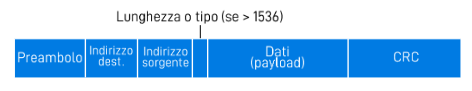
\includegraphics[width=0.6\linewidth]{05/frameEthernet.png}
                \caption{Il \textit{frame} Ethernet}
            \end{figure}
            Il \textit{frame} Ethernet è composto da:
            \begin{description}
                \item[Preambolo] Il preambolo è un campo di 8 byte (0-6: \texttt{10101010}, 7: \texttt{10101011}) che serve per sincronizzare il \textit{clock} dei nodi.
                \item[Indirizzi] L'indirizzo di destinazione e di sorgente sono di 6 byte ciascuno, l'indirizzo di destinazione è l'indirizzo \Acrshort*{MAC} di livello 2 del nodo destinatario, mentre l'indirizzo di sorgente è l'indirizzo \Acrshort*{MAC} del nodo mittente.\footnote{L'indirizzo \Acrshort*{MAC} del destinatario viene inserito prima dell'indirizzo del mittente, questo per permettere ad eventuali nodi intermedi di sapere a chi inoltrare il \textit{frame} senza doverlo decodificare, inoltre se l'indirizzo di destinazione non è per l'host corrente il \textit{frame} viene scartato e il restante del \textit{frame} non viene considerato}
                \item[Tipo] Il campo tipo è di 2 byte e specifica il tipo di protocollo di livello 3 incapsulato nel \textit{frame} Ethernet (ad esempio \Acrshort*{IP}, \texttt{Novell IPX}, \texttt{AppleTalk}, \dots)
                \item[Dati] Il campo dati è di 46-1500 byte e contiene il datagramma di livello 3 incapsulato nel \textit{frame} Ethernet.
                \item[\Acrshort*{CRC}] Il campo \Acrshort*{CRC} è di 4 byte e contiene il codice di rilevamento degli errori.\footnote{Il \Acrshort*{CRC} viene inserito per ultimo in modo che se il \textit{frame} viene scartato a livelli superiori, non venga calcolato il \Acrshort*{CRC} per l'esecuzione del controllo di errore} 
            \end{description}
        \subsubsection{Connessione? \Acrshort*{ACK}, \Acrshort*{NACK}} Ethernet non prevede un meccanismo di conferma di ricezione, e non prevede il mantenimento dello stato della connessione tra due nodi. Questo perché Ethernet è un protocollo di livello 2 \texttt{connectionless} ed inaffidabile. I controlli di questo genere sono demandati a protocolli di livelli superiori.
        \subsubsection{\Acrshort*{CSMA/CD} in Ethernet} 
            L'algoritmo di \Acrshort*{CSMA/CD} in ethernet prevede che:
            \begin{enumerate}
                \item La scheda di rete riceve un datagramma dal livello di rete (3) e lo incapsula in un \textit{frame} Ethernet.
                \item Se una scheda di rete vede il canale libero, trasmette il \textit{frame} intero, altrimenti aspetta finché il canale non è libero.
                \item Se la trasmissione termina senza altre ricezioni la scheda di rete ritiene che il \textit{frame} sia stato trasmesso con successo.
                \item Se ciò non avviene e la scheda di rete rileva una collisione, interrompe la trasmissione e invia un segnale di \textit{abort}.
                \item Dopo una collisione la scheda di rete attende un tempo casuale (\textit{backoff}) tra $0$ e $\left(2^k-1\right)T, k\leq 7$ dove $T$ è il tempo necessario per trasmettere $512$ bit.
            \end{enumerate}
        \subsubsection{Livello fisico e data link} 
            La parte di protocollo \Acrshort*{MAC} è di formato è comune a tutti i protocolli \texttt{\Acrshort*{IEEE} 802.3} ma la parte di livello fisico è diversa. La parte di livello fisico è quella che si occupa di trasmettere i bit sul mezzo trasmissivo, questa parte è diversa per ogni standard \texttt{\Acrshort*{IEEE} 802.3} e per ogni velocità di trasmissione.
\section{\textit{Ethernet Switching}}
    Gli \textbf{\textit{switch}} ethernet sono dispositivi di livello 2 (a differenza degli \textit{hub} che sono di livello 1) che permettono di collegare più nodi in una rete locale. Gli \textit{switch} sono dispositivi che agiscono in modo attivo, memorizzano infatti i \textit{frame} e gli inoltrano, mentre il frame viene inoltrato si analizza il \Acrshort*{MAC} del mittente e si esegue l'associazione porta-\Acrshort*{MAC} in modo da poter inoltrare eventuali \textit{frame} destinati a quel \Acrshort*{MAC} direttamente alla porta associata.\newline
    Inoltre gli \textit{switch} sono trasparenti ai nodi, ovvero i nodi non sanno di essere collegati ad uno \textit{switch} ed inoltre sono \textit{plug-and-play}, ovvero non necessitano di configurazione in quanto vale il principio dell'\textbf{auto-}\textbf{apprendimento}.
    \paragraph{Domini di collisione} Mentre nella tipologia a \Acrshort*{BUS} tutti gli \textit{host} sono sullo stesso ``dominio di collisione'', ovvero ogni nodo può potenzialmente collidere con ogni altro nodo, nella tipologia a \textbf{stella} implementata con degli \textit{switch} ogni \textit{host} è sullo stesso dominio di collisione. Questo in quanto ogni porta dello \textit{switch} è una scheda di rete assestante.
    \paragraph{Trasmissioni simultanee} In una rete \textit{switched} dato che ogni \textit{host} ha un canale dedicato per comunicare con lo \textit{switch} ed il protocollo \textit{ethernet} è applicato individualmente ad ogni porta, è possibile che due \textit{host} trasmettano contemporaneamente senza che si verifichino collisioni, inoltre è possibile che lo \textit{switch} ed l'\textit{host} trasmettano contemporaneamente senza collisioni (In quanto per la trasmissione e la ricezione si usano due doppini separati).
    \subsection{AutoApprendimento - \textit{backward learning}}
        Gli \textit{switch} Ethernet grazie ad una tabella che associa \Acrshort*{MAC} del destinatario ad una interfaccia di uscita, sono in grado di inoltrare i \textit{frame} diretti a quel \Acrshort*{MAC} direttamente alla porta associata, il tutto senza dover inoltrare il \textit{frame} a tutte le porte e/o doverlo memorizzare. Per compilare questa tabella si usa il \textit{backward learning}, che consiste nel ``leggere'' il \Acrshort*{MAC} del mittente di ogni pacchetto in entrata e memorizzarlo nella tabella associandolo alla porta di ingresso, se il \Acrshort*{MAC} di destinazione non è presente nella tabella si inoltra il \textit{frame} a tutte le porte tranne a quella di ingresso. Quando il \textit{frame} arriva al destinatario se questo risponde, il \textit{frame} viene letto ed il \Acrshort*{MAC} del destinatario viene memorizzato nella tabella associandolo alla porta di ingresso.
        \paragraph{Filtro inoltro} Nel caso nel quale un \textit{frame} arrivi ad uno \textit{switch} e il \Acrshort*{MAC} di destinazione sia presente nella tabella, il \textit{frame} viene inoltrato solo alla porta associata al \Acrshort*{MAC} se questa è diversa dalla porta di ingresso, altrimenti il \textit{frame} viene scartato. Questo accade per mantenere la retro-compatibilità con le reti \textit{hub-ed}. Se invece il \Acrshort*{MAC} di destinazione non è presente nella tabella, viene eseguito il \textit{flooding}.
        \paragraph{Con \textit{switch} multipli} Nel caso di \textit{switch} multipli organizzati ad \textit{albero} la situazione non cambia molto, infatti ogni \textit{switch} esegue il \textit{flooding} se il \Acrshort*{MAC} di destinazione non è presente nella tabella, altrimenti inoltra il \textit{frame} alla porta associata al \Acrshort*{MAC} se questa è diversa dalla porta di ingresso, altrimenti il \textit{frame} viene scartato.
        \paragraph{\textit{Switch} in anello} Nel caso di \textit{switch} collegati in anello si possono verificare dei problemi di \textit{loop}, infatti se viene eseguito il \textit{flooding} da un \textit{switch} ad un altro \textit{switch} e questo \textit{switch} inoltra il \textit{frame} ad un terzo \textit{switch} che lo inoltra al primo \textit{switch} si crea un \textit{loop}. Questo genere di \textit{loop} saturano la rete e portano ad un sovraccarico degli apparati. Per evitare questo genere di problemi si usano topologie di rete differenti. Oppure si usano protocolli di \textit{loop prevention} come il \acrfull*{STP}.
    \subsection{\textit{Spanning tree} per \textit{switch}}
        In quanto in reti complesse si usano più connessioni tra due switch e/o tra switch e \textit{host} si possono creare dei \textit{loop} viene introdotto il protocollo \textbf{\textit{Spanning Tree Protocol}}. Questo protocollo prevede che i vari \textit{switch} abbaino un numero identificativo univoco di $64$ bit per il quale i primi $16$ bit sono impostati dall'amministratore di rete ed i restanti $48$ bit è il \Acrshort*{MAC} dello \textit{switch}. Questo numero viene usato per determinare quale \textit{switch} è il \textit{root} della rete. Il \textit{root} è lo \textit{switch} con il numero più basso.\newline
        Se infatti è probabile la presenza di \textit{loop} allora gli \textit{switch} si scambiano messaggi contenenti l'\Acrshort*{ID} dello \textit{switch} ed il costo del \textit{link}, quando uno \textit{switch} riceve un \acrfull*{BPDU} controlla gli \Acrshort*{ID} nella sua tabella e se il nuovo \Acrshort*{ID} è più basso allora la porta sul quale è arrivato il \Acrshort*{BPDU} diventa la porta di uscita per il \textit{root}, altrimenti la porta viene bloccata. Questo processo viene ripetuto per ogni \textit{switch} e per ogni porta.
        \paragraph{Variazioni} Se un \textit{link} si rompe o si crea un nuovo \textit{link} allora il processo di determinazione del \textit{root} viene ripetuto, ciò accade o in modo automatico, tramite l'invio periodico di \Acrshort*{BPDU} alle porte \textit{designated}, da notare come ogni \Acrshort*{BPDU} ricevuta abbia un \Acrshort*{TTL} che invecchia ad ogni secondo. Se il \Acrshort*{TTL} arriva a $0$ allora il \textit{link} viene considerato morto e il processo di determinazione del \textit{root} viene ripetuto. 
        \paragraph{Performance} Il protocollo non esclude che possano esserci percorsi più lunghi del necessario, ciò può accadere se il \textit{root} non viene impostato ``intelligentemente'' e se la topologia della rete è complessa. 
        \paragraph{Dominio di \textit{broadcast} v/s collisione} 
            \begin{definition}[Dominio di collisione]
                Si definisce con il termine \textbf{dominio di collisione} in una rete, quella parte tale per cui se due o più \textit{nodi} trasmettono in maniera simultanea, allora si verifica una collisione.
            \end{definition}
            \begin{definition}[Dominio di \textit{broadcast}]
                Si definisce con il termine \textbf{dominio di \textit{broadcast}} in una rete, quella parte tale per cui se un nodo trasmette un \textit{frame} del tipo \textit{broadcast} di livello 2, allora tutti i nodi presenti nel dominio ricevono il \textit{frame}.
            \end{definition}
    \subsection[\textit{Virtual Local Area Network} (\texttt*{VLAN})]{\acrfull*{VLAN}}
        Se si vuole dividere una rete \Acrshort*{LAN} in più reti diverse per necessità di separazione di intenti, carico o per separare i domini di \textit{broadcast} si possono usare le \textbf{VLAN} (\textit{Virtual Local Area Network}).\newline
        Le \Acrshort*{VLAN} sono reti logiche che permettono di separare i nodi in base al \Acrshort*{MAC} in gruppi logici, in modo che i nodi appartenenti ad una \Acrshort*{VLAN} possano comunicare tra loro come se fossero collegati ad una rete fisica separata anche attraverso a \textit{switch} diversi.\newline
        Non tutti gli \textit{switch} però possono supportare le \Acrshort*{VLAN}, infatti per poter supportare le \Acrshort*{VLAN} uno \textit{switch} deve supportare il protocollo \texttt{\Acrshort*{IEEE} 802.1Q} che permette di aggiungere un \textit{tag} al \textit{frame} Ethernet che specifica a quale \Acrshort*{VLAN} appartiene il \textit{frame} stesso.\newline
        Il vantaggio delle \Acrshort*{VLAN} è che permettono di separare i domini di \textit{broadcast} e di \textit{collisione} mantenendo comunque la possibilità di comunicare tra le varie \Acrshort*{VLAN} attraverso più \textit{switch} differenti, infatti gli \textit{switch} che supportano le \Acrshort*{VLAN} sono in grado di inoltrare i \textit{frame} tra di loro configurando i \textit{link} come \textit{trunk} ovvero \textit{link} che trasportano più \Acrshort*{VLAN} contemporaneamente. Inoltre gli \textit{host} non sono \texttt{VLAN-aware} ovvero non sanno a quale \Acrshort*{VLAN} appartengono e di conseguenza riducono la complessità di configurazione della rete.\newline
        Quest'ultima caratteristica rende le \Acrshort*{VLAN} retro-compatibili con tutti i dispositivi \textit{host}, mentre per gli \textit{switch} è necessario che supportino il protocollo o che almeno ne conoscano il funzionamento, difatti se uno \textit{switch} che non supporta le \Acrshort*{VLAN} riceve un \textit{frame} con un \textit{tag} \Acrshort*{VLAN} questo \textit{frame} viene scartato e/o inoltrato come un normale \textit{frame} Ethernet. Per ovviare ciò è necessario configurare la porta di uscita verso quello \textit{switch} come se fosse un normale \textit{host}, in questo caso tutti gli \textit{host} collegati a quello \textit{switch} appartengono alla stessa \Acrshort*{VLAN}.
\section[\texttt{IEE 802.11} - \texttt{Wi-Fi}]{\texttt{\Acrshort*{IEEE} 802.11} - \Acrshort*{Wi-Fi}}
    \subsection{Terminologia ed architettura}
        \begin{definition}[Host Wireless]
            Si definisce con il termine \textbf{\textit{host wireless}} un dispositivo che può trasmettere e ricevere dati tramite onde radio. Questi possono essere sia statici che mobili.
        \end{definition}
        \begin{definition}[Stazione Base]
            Si definisce con il termine \textbf{stazione base} un dispositivo che, tipicamente connesso ad una rete cablata, esegue il \textit{relay} dei dati tra gli \textit{host} \textit{wireless} e la rete cablata.
        \end{definition}
        \begin{definition}[Collegamento \textit{wireless}]
            Si definisce con il termine \textbf{collegamento \textit{wireless}} l'insieme del collegamento senza fili tra un \textit{host} \textit{wireless} ed una stazione base ed il protocollo \Acrshort*{MAC} che regola l'accesso al mezzo trasmissivo.
        \end{definition}
        \begin{definition}[Modalità infrastrutturata]
            Si definisce con il termine \textbf{modalità infrastrutturata} una modalità di funzionamento di una rete \textit{wireless} nella quale gli \textit{host} \textit{wireless} comunicano tra di loro attraverso una stazione base. Inoltre il processo di \textit{handover} tra più stazioni base è trasparente agli \textit{host}.
        \end{definition}
        \begin{definition}[Modalità ad hoc]
            Si definisce con il termine \textbf{modalità ad hoc} una modalità di funzionamento di una rete \textit{wireless} nella quale non sono presenti stazioni base e gli \textit{host} \textit{wireless} comunicano direttamente tra di loro. Questi possono trasmettere solo ad altri \textit{host} \textit{wireless} che si trovano nel loro raggio di copertura, oppure possono essere determinati dei protocolli detti multi-salto che permettono di trasmettere ad \textit{host} che non sono direttamente raggiungibili.
        \end{definition}
        \subsubsection{Standard \texttt{\Acrshort*{IEEE} 802.11}}
            Lo standard \texttt{\Acrshort*{IEEE} 802.11} definisce i protocolli di livello 2 e 1 per le reti \textit{wireless}. Esistono molte varianti di questo standard, le più comuni sono:
            \begin{description}
                \item[\texttt{802.11b}] $2.4-5.8GHz$ fino ad un massimo di $11Mbps$ ed protocollo simile ad \Acrshort*{CDMA}.
                \item[\texttt{802.11a}] $5-6GHz$ fino ad un massimo di $54Mbps$
                \item[\texttt{802.11g}] $2.4-5.8GHz$ fino ad un massimo di $54Mbps$
                \item[\texttt{802.11n}] Antenne multiple, $2.4-5.8GHz$ con range di velocità da $72$ a $600Mbps$ per tre flussi contemporanei.
                \item[\texttt{802.11ac}] canali con più banda e più flussi, $5GHz$ con velocità fino a $6.9Gbps$ con 4 flussi contemporanei.
                \item[\texttt{802.11ax}] meglio conosciuto come \texttt{\Acrshort*{Wi-Fi} 6}, $2.4-5.8GHz$ con velocità fino a $11Gbps$ per 8 flussi contemporanei, quindi $1375Mbps$ per ogni stazione.
            \end{description}
        \subsubsection{Architettura in una rete \Acrshort*{WLAN}}
            Un una architettura di base di una rete \Acrshort*{WLAN} si hanno una stazione \textit{wireless} \acrfull*{STA} (o anche \textit{nodo}) che tramite un \acrfull*{BSS} che è un gruppo di \Acrshort*{STA} che usano lo stesso canale radio alla quale fà parte un \acrfull*{AP} che è una stazione integrata nella \Acrshort*{LAN} cablata attraverso un \acrfull*{DS} che fornisce connettività verso o altri \Acrshort*{BSS} oppure verso \textit{internet}, l'unione che il \Acrshort*{DS} crea tra più \Acrshort*{BSS} è chiamata \acrfull*{ESS}, infine il \textit{Portal} a monte del \Acrshort*{DS} è l'entità che fornisce connettività verso l'esterno.\newline
            In tutto questo un \Acrshort*{BSS} può essere isolato o connesso tramite un \Acrshort*{AP} il quale solitamente gestisce il protocollo \Acrshort*{MAC} e la gestione del canale radio, all'interno di un \Acrshort*{ESS} possono essere presenti più \Acrshort*{AP} con protocolli \Acrshort*{MAC} differenti.
        \subsubsection{\texttt{802.11}}
            \paragraph{Canali e assocazione} In una rete \texttt{802.11b} lo spettro di frequenza da $2.4GHz$ a $2.485GHz$ è diviso in $11$ canali (o $14$ se sussistono particolari condizioni), è dunque l'amministratore di quell'\Acrshort*{AP} a scegliere il canale, solitamente sulla presenza o meno di altri \Acrshort*{AP} vicini e sulla presenza o meno di interferenze. Quando un \Acrshort*{STA} deve associarsi ad un \Acrshort*{AP} ascolta i messaggi di \texttt{beacon} inviati da tutti gli \Acrshort*{AP} i quali contengono informazioni sul nome \acrfull*{SSID} e l'indirizzo \Acrshort*{MAC} dell'\Acrshort*{AP}. Allora la \Acrshort*{STA} sceglie l'\Acrshort*{AP} tra l'elenco di quelli disponibili, si associa ad esso (se necessario si autentica), usa il protocollo \Acrshort*{DHCP} per ottenere un indirizzo \Acrshort*{IP} e poi può comunicare con la rete.
            \paragraph{Scansione attiva e passiva} Nel processo di associazione distinguiamo la scansione attiva da una passiva: in una scansione passiva l'\textit{host} ascolta i \textit{beacon} degli \Acrshort*{AP} ed l'\textit{host} con quale associarci, l'\Acrshort*{AP} risponde con un messaggio di conferma. Nella scansione attiva invece l'\textit{host} invia a tutti gli \Acrshort*{AP} un messaggio di \textit{probe request} e l'\Acrshort*{AP} risponde con un messaggio di \textit{probe response}, successivamente l'\textit{host} si associa all'\Acrshort*{AP} scelto con la solita procedura.
        \subsubsection{Caratteristiche dei collegamenti \textit{wireless}}
            A differenza delle connessioni cablate, le connessioni \textit{wireless} sono molto più soggette a interferenze, infatti telefoni, forni a microonde o altri usano la stessa frequenza di $2.4GHz$ e possono interferire con la connessione. Inoltre la presenza di ostacoli come muri, mobili o persone può ridurre la qualità e l'intensità del segnale. Inoltre è possibile che lo stesso segnale raggiunga la stazione ricevente in modo diverso, infatti il segnale può essere riflesso, rifratto o assorbito.\newline
            Tutto ciò insieme al fatto che l'attenuazione delle onde radio segue una legge quadratica inversa alla distanza rende la \textit{collision detection} impossibile. Legato allo stesso problema sussiste il fatto che una antenna non può trasmettere e ricevere contemporaneamente (auto-interferenza) e che due antenne vicine possono interferire tra di loro (interferenza tra antenne).
    \subsection[Protocolli \texttt{MAC}]{Protocolli \Acrshort*{MAC}}
        In quanto come descritto precedentemente la \textit{collision detection} è impossibile, si usano protocolli \Acrshort*{MAC} differenti che si basano su \Acrfull*{CSMA/CA}. Questo protocollo prevede che le \Acrshort*{STA} che necessitano di trasmettere si contendano il canale radio, ogni volta che una \Acrshort*{STA} ha qualcosa da trasmettere ripete la contesa con le altre \Acrshort*{STA}. Sono presenti tuttavia delle eccezioni a ciò, infatti in versioni più avanzate di \texttt{802.11} (come \texttt{802.11n/ac/ax}) si possono concedere periodi più lunghi rispetto alla lunghezza del frame. Questo viene chiamato \Acrfull*{TXOP} e permette di trasmettere più frame in un unico periodo di tempo.
        \subsubsection{Trasmettitore \Acrshort*{CSMA}}
            Il trasmettitore \Acrshort*{CSMA} funziona nel seguente modo:
            \begin{enumerate}
                \item Se il canale rimane libero per un tempo \acrfull*{DIFS} allora la \Acrshort*{STA} può trasmettere. Altrimenti entra in \textit{backoff}.
                \item Se il canale è occupato allora:
                    \subitem si sceglie un tempo di \textit{backoff} casuale
                    \subitem quando il tempo di \textit{backoff} è scaduto e il canale è libero si trasmette solo quando il timer è scaduto.
            \end{enumerate}
            Se non si riceve nessun \Acrshort*{ACK} allora si aumenta il valore massimo del tempo di \textit{backoff} e si sceglie un nuovo tempo di \textit{backoff} casuale.\newline
            Se invece il messaggio viene ricevuto correttamente si attende un tempo \acrfull*{SIFS} \footnote{\Acrshort*{DIFS}>\Acrshort{SIFS} per evitare altre trasmissioni di altri \textit{host}} e si invia un \Acrshort*{ACK} al mittente. In questo protocollo \Acrshort*{MAC} gli \Acrshort*{ACK} sono necessari per garantire la corretta ricezione del messaggio e per le eventuali collisioni dopo il tempo di \textit{backoff} in quanto il mittente non può ascoltare il canale mentre trasmette.
            \paragraph{Problema del terminale nascosto} Il problema del terminale nascosto è un problema che si verifica quando due \Acrshort*{STA} non possono ascoltare il canale tra di loro e quindi non possono sapere se il canale è libero o occupato. Ovvero assumiamo la situazione dove gli host \texttt{A} e \texttt{B} sono nel range di comunicazione, inoltre \texttt{B} e \texttt{C} possono comunicare tra di loro sullo stesso canale, in questa situazione ne \texttt{A} ne \texttt{C} possono sapere se il canale è libero o occupato. Questo problema può essere risolto con l'uso di \Acrshort*{CSMA/CA} con \textit{handshaking}.
        \subsubsection{\Acrshort*{MAC} con messaggi \Acrshort*{RTS}/\Acrshort*{CTS}}
            In questa situazione si aggiunge una procedura di \textit{handshaking} dove il trasmettitore deve inviare un messaggio di \acrfull*{RTS} e il ricevitore se è libero risponde con un messaggio di \acrfull*{CTS}. Questo permette di risolvere il problema del terminale nascosto e di evitare collisioni. Questo metodo però introduce un ritardo aggiuntivo dovuto alla trasmissione dei messaggi di \Acrshort*{RTS} e \Acrshort*{CTS}. Nel momento in cui il trasmettitore riceve il messaggio di \Acrshort*{CTS} può trasmettere il messaggio ed il canale viene riservato per la trasmissione del messaggio.
            \paragraph{Problema del terminale esposto} Il problema del terminale esposto è un problema che si verifica quando si usa un protocollo di \textit{handshaking} e due \textit{host} vogliono comunicare con due \Acrshort*{AP} diversi. In questo caso il \textit{host} \texttt{A} invia un messaggio di \Acrshort*{RTS} al \Acrshort*{AP} \texttt{X} il quale invierà un messaggio di \Acrshort*{CTS} di fatto bloccando il canale anche per l'\Acrshort*{AP} \texttt{Y} che si trova nelle vicinanze. Allora l'host \texttt{B} dovrà aspettare l'\Acrshort*{ACK} del \Acrshort*{AP} \texttt{X} che libera l'\Acrshort*{AP} \texttt{Y} e quindi il canale.
    \subsection{Frame ed indirizzi \texttt{802.11}}
        \begin{figure}[H]
            \centering
            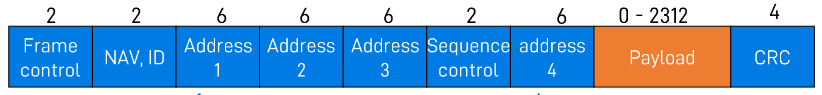
\includegraphics[width=0.6\linewidth]{05/frame802.11.png}
            \caption{Il \textit{frame} \texttt{802.11}}
        \end{figure}
        Possiamo notare che oltre ai campi classici di un \textit{frame} Ethernet, il \textit{frame} \texttt{802.11} contiene:
        \begin{description}
            \item[\textit{Address 1}] L'indirizzo \Acrshort*{MAC} del destinatario \textit{wireless}
            \item[\textit{Address 2}] L'indirizzo \Acrshort*{MAC} del mittente \textit{wireless}
            \item[\textit{Address 3}] L'indirizzo \Acrshort*{MAC} del \textit{router} al quale è collegato l'\Acrshort*{AP} (destinatario \Acrshort*{LAN})
            \item[\textit{Sequence Control}] Il numero di sequenza del \textit{frame}
            \item[\textit{Address 4}] L'indirizzo \Acrshort*{MAC} del mittente \textit{wireless} (usato solo in modalità ad hoc)
        \end{description}
        Questi quattro indirizzi sono usati per permettere la comunicazione tra \Acrshort*{STA} e \Acrshort*{AP} e per permettere la comunicazione tra \Acrshort*{STA} in modalità ad hoc.